\documentclass{article}
\usepackage{graphicx}
%permite ecribir acentos directamente
\usepackage[utf8]{inputenc}
% Esto es para que el LÁTEX sepa que el texto está en español, se agrega el ingles para el paquete de gráfico de circuitos:
\usepackage[spanish]{babel}
\usepackage{geometry}
 \geometry{a4paper,total={170mm,257mm},left=25mm,right=25mm,top=20mm,}
\usepackage{hyperref} 
\usepackage{amsmath, amsfonts}
\usepackage{enumitem}
\usepackage{xcolor}
\usepackage{textcomp}
\usepackage{fancyhdr}

\pagestyle{fancy}
\fancyhf{}
\lhead{Medidas Electrónicas II}
\rhead{Simulación y análisis de distintas fibras ópticas}
\rfoot{Página \thepage}

\usepackage{pgfplots}
\usepackage{pgfplotstable}
\usepackage{booktabs}
\usepackage{array}
\usepackage{colortbl}

\pgfplotstableset{% global config, for example in the preamble
  every head row/.style={before row=\toprule,after row=\midrule},
  every last row/.style={after row=\bottomrule},
  fixed,precision=1,
}

\begin{document}
\begin{titlepage}
 \centering
	
\includegraphics[scale=0.80]{imagenes/LOGO.jpg} \par
 	\vspace{1cm}
 	{\scshape\LARGE Universidad Tecnológica Nacional \par}
 	{\scshape\large Facultad Regional de Córdoba \par}
 	\vspace{1cm}
	{\bfseries \Large Trabajo Práctico de simulación\par}
	{\bfseries \large Simulación y análisis de distintas fibras ópticas \par}
 	\vspace{1.5cm}

	\begin{tabular}{ll}

		Navarro, Facundo 	&	63809 	\\
	\end{tabular}
	
	\vspace{1cm}
	Curso: 5r2 \\
 	\vfill
	{\bfseries \Large Medidas Electrónicas II \par}

	\vspace{1.5cm}
	Docentes: \par
	Ing. Martinez, Denis \par

 	\vfill
	{\large \today\par}
\end{titlepage}

%##################################### INDICE  #####################################################

\tableofcontents
\clearpage

%##################################### INDICE  #####################################################

\section{Introducción}
La fibra óptica es un medio de transmisión empleado habitualmente en redes de datos; un hilo muy fino de material transparente, vidrio o materiales plásticos, por el que se envían pulsos de luz que representan los datos a transmitir. Las fibras se utilizan ampliamente en telecomunicaciones, ya que permiten enviar gran cantidad de datos a gran velocidad, mucho más rápido que en las comunicaciones de radio y cable. También se utilizan para redes locales. Son el medio de transmisión por excelencia, inmune
a las interferencias pero por otro lado se puede decir como aspecto negativo que tienen un costo elevado.

Un OTDR es un probador de fibra óptica que se utiliza para categorizar redes de fibra óptica para telecomunicaciones. La finalidad de un OTDR es detectar, localizar y medir elementos en cualquier ubicación de un enlace de fibra óptica. Un OTDR necesita acceder únicamente a una terminación del enlace y actúa como un sistema de radar de una sola dimensión. Al proporcionar señales gráficas de las fibras sometidas a prueba, es posible obtener una representación gráfica de todo el enlace de fibra ópica

El OTDR emite un tren de señales pulsadas en la fibra, en cuyo interior tiene lugar una serie de incidencias debidas a conectores, empalmes, irregularidades, curvaturas y defectos. El OTDR analiza el retorno de señal debido a estas reflexiones, sean debidas a efecto Fresnel o Rayleight.

Las reflexiones de Fresnel son debidas la variación de la velocidad de la luz en unción del medio atravesado, y la retrodispresión de Rayleight se corresponde con las impurezas u otro tipo de incidentes internos de la fibra.

Estas señales, detectadas por el foto detector de avalancha (APD) del equipo, permiten al técnico el trazado de una gráfica de señal recibida con relación al pulso inyectado en la fibra. A partir de ella, el OTDR determina el final de la fibra.

\section{Simulación}
Por practicidad se procede a simular con el software \textbf{uOTDR} que incluye muchos tipos de fibras para analizar, ya que en realidad se necesita de un hardware externo para poder realizar mediciones sobre fibras ópticas reales.


\subsection{Traza b409m}

\begin{figure}[h]
 \begin{center}
	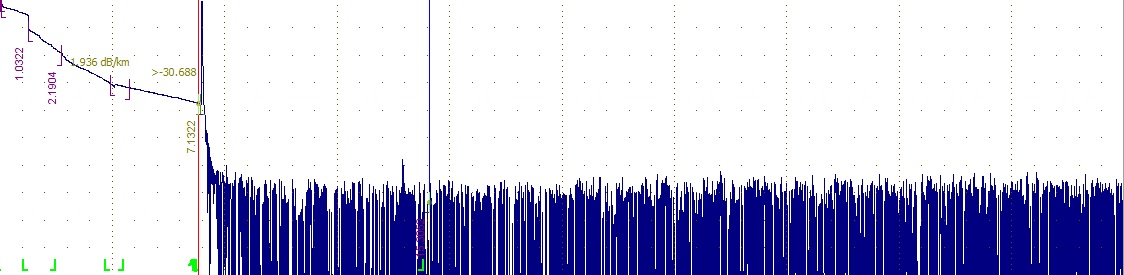
\includegraphics[width=\textwidth]{imagenes/sim1.jpg} 
	\caption{Traza b409m}\label{fig:fig1}
 \end{center}
\end{figure}

\begin{itemize}\itemsep0em \itemindent=2em
\item Resolución X: 40.0072 [Km/div]
\item Resolución Y:	36.115 [dB/div]
\item Tipo de fibra: MM-1310
\item Indice de refractancia: 1.47500
\item Distancia máxima: 40 [km]
\item Ancho de pulso: 90 [ns]
\item Atenuación completa: 37.015 [dB]
\item Pérdida óptica de retorno: 59.5588 [dB]
\item Coeficiente de reflexión: -30.673 [dB]
\end{itemize}

\begin{itemize}\itemsep0em \itemindent=2em
\item[•]Eventos:
	\begin{itemize}\itemsep0em \itemindent=2em
		\item[*] 0 m 	 : Conector incial.
		\item[*] 1,03 km : Pérdida por fusión.
		\item[*] 2,19 km : Pérdida por empalme.
		\item[*] 3,91 Km : Fisura.
		\item[*] 7,13 Km : Terminación de la fibra.
		\item[*] >7,13Km : Ruidos.
	\end{itemize}
\end{itemize}

\subsection{Traza 3km-mm}

\begin{figure}[h]
 \begin{center}
	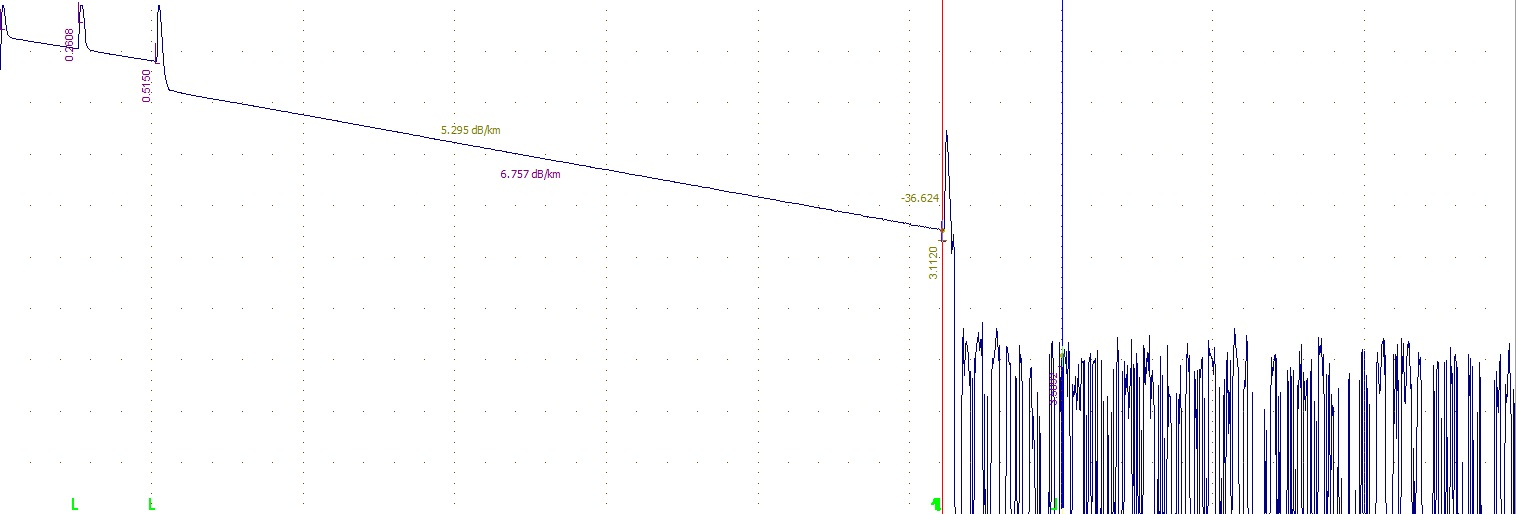
\includegraphics[width=\textwidth]{imagenes/sim2.jpg} 
	\caption{Traza 3km-mm}\label{fig:fig1}
 \end{center}
\end{figure}

\begin{itemize}\itemsep0em \itemindent=2em
\item Resolución X: 5.0047 [Km/div]
\item Resolución Y:	3.611 [dB/div]
\item Tipo de fibra: MM-850
\item Indice de refractancia: 1.47500
\item Distancia máxima: 5.0 [km]
\item Ancho de pulso: 330 [ns]
\item Atenuación completa: 8.798 [dB]
\item Pérdida óptica de retorno: 52.779 [dB]
\item Coeficiente de reflexión: -36.658 [dB]
\end{itemize}


\begin{itemize}\itemsep0em \itemindent=2em
\item[•]Eventos:
	\begin{itemize}\itemsep0em \itemindent=2em
		\item[*] 0 m 	 : Conector incial.
		\item[*] 260,8 m : Pérdida por conector.
		\item[*] 515,0 m : Pérdida por conector.
		\item[*] 3,12 Km : Terminacion de la fibra.
		\item[*] >3,12Km : Ruidos.
	\end{itemize}
\end{itemize}


\subsection{Traza 100km.sor}

\begin{figure}[h]
 \begin{center}
	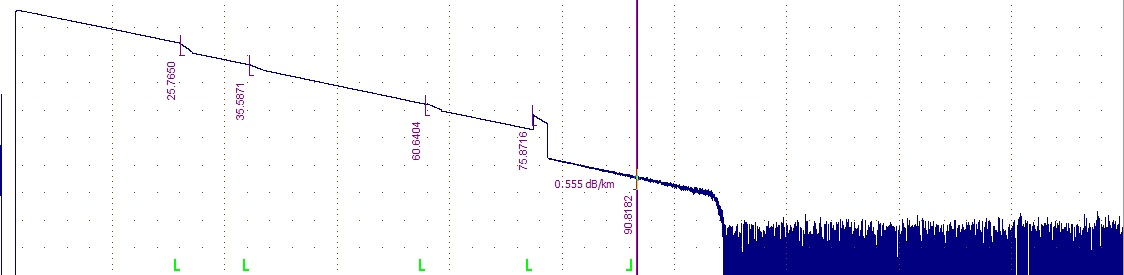
\includegraphics[width=\textwidth]{imagenes/sim3.jpg} 
	\caption{Traza 100km}\label{fig:fig1}
 \end{center}
\end{figure}

\begin{itemize}\itemsep0em \itemindent=2em
\item Resolución X: 16000 [Km/div]
\item Resolución Y:	3.612 [dB/div]
\item Tipo de fibra: SM-1550
\item Indice de refractancia: 1.46820
\item Distancia máxima: 160 [km]
\item Ancho de pulso: 20 [us]
\item Atenuación completa: 16.118 [dB]
\item Pérdida óptica de retorno: 95.371 [dB]
\item Coeficiente de reflexión: -64.002 [dB]
\end{itemize}

\begin{itemize}\itemsep0em \itemindent=2em
\item[•]Eventos:
	\begin{itemize}\itemsep0em \itemindent=2em
	\item[*] 25,7 Km : Pérdida por fusión.
	\item[*] 35,5 Km : Pérdida por dobladura.
	\item[*] 60,6 Km : Pérdida por dobladura.
	\item[*] 75,8 Km : Terminacion de la fibra.
	\item[*] >75,8Km : Ruidos.
\end{itemize}
\end{itemize}
\end{document}